\documentclass[11pt,a4paper]{article}

% ==========================================
% arXiv-Safe Preamble
% ==========================================
\usepackage[utf8]{inputenc}
\usepackage[T1]{fontenc}
\usepackage{amsmath,amssymb,amsthm}
\usepackage{graphicx}
% Hyperref: Inline configuration to avoid conflicts
\usepackage[colorlinks=true,linkcolor=blue,citecolor=blue,urlcolor=blue]{hyperref}
\usepackage[numbers]{natbib}
\usepackage{geometry}
\usepackage{booktabs}
\usepackage{caption}

% Page geometry
\geometry{
  left=2.5cm,
  right=2.5cm,
  top=2.5cm,
  bottom=2.5cm
}

% Custom commands
\newcommand{\AneqAapproxA}{A \neq A \approx A}

% Title and author
\title{\textbf{NRR-Core: Non-Resolution Reasoning as a Computational Framework for Contextual Identity and Ambiguity Preservation}}

\author{
  Kei Saito\thanks{ORCID: 0009-0006-4715-9176} \\
  Independent Researcher, Japan \\
  \texttt{kei.saito.research@gmail.com}
}

\date{December 2025 \\[0.5em]
\textit{Part of the Non-Resolution Reasoning (NRR) research program.}}

\begin{document}

\maketitle

\begin{center}
\textcopyright\ 2025 Kei Saito.
Licensed under CC BY 4.0.\\
\url{https://creativecommons.org/licenses/by/4.0/}
\end{center}

\begin{abstract}
Current artificial intelligence systems, despite remarkable capabilities in text generation and pattern recognition, exhibit a fundamental architectural limitation: they resolve ambiguity prematurely.
This premature semantic collapse---the tendency to collapse multiple valid interpretations into a single output---stems from classical identity assumptions embedded in standard neural architectures.
We propose \textbf{Non-Resolution Reasoning (NRR)}, a computational framework that treats ambiguity retention as a valid reasoning mode rather than a defect to be eliminated.
NRR introduces three core principles: (1) \textbf{Non-Identity ($A \neq A$)}---the same symbol refers to different entities across contexts;
(2) \textbf{Approximate Identity ($A \approx A$)}---entities share partial structural overlap without being identical;
and (3) \textbf{Non-Resolution}---conflicting interpretations can coexist without forced convergence.
We formalize these principles through three architectural components: \textbf{Multi-Vector Embeddings} for context-dependent representation, \textbf{Non-Collapsing Attention} for parallel interpretation retention, and \textbf{Contextual Identity Tracking (CIT)} for maintaining $A \neq A$ across inference.
We provide functional verification of the Multi-Vector Embeddings component through a controlled synthetic task.
We illustrate NRR's potential through case studies in paradox handling, creative generation, and context-dependent reasoning.
Crucially, we provide functional verification in a synthetic two-turn disambiguation task through a Turn 1 Entropy measurement demonstrating ambiguity preservation directly: NRR-lite maintains high entropy ($H = 0.91$ bits, near-maximum $1.0$) at the ambiguous turn, while standard architectures collapse early ($H = 0.15$ bits), demonstrating that NRR preserves interpretive flexibility until context arrives.
NRR challenges the assumption that meaning must collapse to be useful, offering a foundation for AI systems capable of sophisticated ambiguity handling and creative reasoning.
\textbf{The question is not whether AI should resolve ambiguity, but when, how, and under whose control.}

\textbf{Implementation}: A reference implementation accompanying this work 
is available at \url{https://github.com/kei-saito-research/nrr-core}.
\end{abstract}

\noindent\textbf{Keywords:} Non-resolution reasoning, contextual identity, ambiguity preservation, multi-vector embeddings, non-collapsing attention, entropy measurement

\section{Introduction}

This paper is one module in an ongoing Non-Resolution Reasoning (NRR) research program, not a closed endpoint. Companion papers cover text-to-state mapping, implementation strategy, and cross-domain validation with distinct scopes. A series-level Program Map and update status will be maintained in repository documentation.

\subsection{Series Alignment: Notation and Metrics}

\textbf{Notation contract.} In this paper, $\sigma$ and $\delta$ denote the
\emph{state-level} operator family in the foundational formalism. Later
implementation papers use item-level update operators
($\sigma_{\text{item}}, \delta_{\text{item}}$). The symbol family is shared, but
the abstraction level differs by design; direct one-to-one interpretation
requires explicit subscripts.

\textbf{Metric contract.} Core focuses on \emph{foundational non-collapse}
metrics (e.g., Turn-1 entropy under ambiguity). Later papers add interface and
operational metrics (e.g., extraction reliability, token efficiency, and
stability). These are complementary measurement layers, not replacements of the
foundational criterion.

\textbf{Boundary statement.} Claims in this paper are limited to the tested
functional verification setup and foundational formalization scope.

\subsection{The Problem of Premature Semantic Collapse}

Large language models (LLMs) have achieved remarkable success in natural language processing \cite{devlin2019bert, radford2018improving}, demonstrating fluency in text generation, translation, and question-answering.
However, these systems share a fundamental limitation: they over-commit to early resolution of ambiguity.
This ``premature semantic collapse bias'' manifests as:

\begin{itemize}
\item Binary decisions forced too quickly
\item Collapse of multiple valid interpretations into single outputs
\item Overconfident inference in uncertain contexts
\item Unnecessary computational branching and backtracking
\item Brittleness when handling paradoxes and self-referential structures
\end{itemize}

The root cause lies in classical identity assumptions embedded in neural architectures.
Standard embedding layers assign each token a fixed vector (or context-dependent but ultimately collapsed representation \cite{peters2018deep}).
Attention mechanisms use softmax normalization \cite{vaswani2017attention}, forcing probabilistic collapse to sum-to-one distributions.
Generation objectives optimize for single ``correct'' outputs rather than maintaining interpretation flexibility.
While recent decoding strategies introduce diversity at the output level \cite{holtzman2020curious, li2023contrastive}, the underlying representations still collapse internally.

Yet human cognition operates differently.
Humans routinely maintain multiple interpretations simultaneously, suspend judgment when context is insufficient, and navigate contradictions without forcing resolution.
This discrepancy suggests that AI's struggles with ambiguity, paradox, creativity, and nuanced reasoning stem not from insufficient data or model scale, but from \textbf{architectural assumptions about how meaning should be processed}.

Several lines of prior work address related aspects of these limitations without targeting the core collapse problem.
Efficient attention variants \cite{child2019generating, dao2022flashattention} reduce computational cost but retain softmax normalization and its inherent collapse pressure.
Mixture-of-experts architectures \cite{shazeer2017outrageously} maintain parallel computational pathways but route inputs to single experts, enforcing collapse at the routing level.
Probabilistic programming languages \cite{goodman2008church} maintain distributions over hypotheses but typically aim for eventual convergence to point estimates.
Neurosymbolic approaches \cite{garcez2020neural} integrate logical and neural reasoning but inherit classical identity assumptions from their symbolic components.
NRR differs from all of these by treating non-resolution---the sustained coexistence of conflicting interpretations---as a first-class computational primitive.

\subsection{Contributions of This Work}

This paper introduces Non-Resolution Reasoning (NRR), a computational framework that treats non-resolution---the deliberate maintenance of undecided states---as a valid and computationally useful reasoning mode.
Our contributions are:

\begin{enumerate}
\item \textbf{Conceptual Framework}: We formalize three core principles (Non-Identity, Approximate Identity, Non-Resolution) that challenge classical identity assumptions in AI reasoning.
\item \textbf{Architectural Components}: We propose three implementable mechanisms---Multi-Vector Embeddings, Non-Collapsing Attention, and Contextual Identity Tracking (CIT)---adaptable to existing neural architectures.
\item \textbf{Functional Verification}: We validate ambiguity preservation directly via Turn 1 Entropy measurement, showing NRR-lite maintains $H = 0.91$ bits (near-maximum) while the baseline collapses to $H = 0.15$ bits, consistently across five random seeds.
\item \textbf{Theoretical Formalization}: We provide a mathematical outline, including a formal state space, a compact core operator set for non-collapsing transitions, and extensible metadata functions for context tracking, with explicit formalization of the $\AneqAapproxA$ principle.
\item \textbf{Implementation Roadmap}: We provide concrete benchmarking strategies and computational cost considerations to enable validation and extension.
\end{enumerate}

Contribution type and claim boundary are explicit: this work does not claim novelty of ambiguity-aware behavior in human reasoning, nor universal superiority of NRR over all alternatives. The contribution is to operationalize tacit ambiguity-management practices into a reproducible, testable, and deployable protocol with explicit boundary/failure reporting under tested conditions.
NRR is anti-premature-collapse, not anti-collapse: commitment remains necessary, but commitment timing must be condition-designed rather than fixed by default.
This design concerns decision structure rather than interpersonal tone: outputs may remain concise/direct while still preserving conditional optionality until fixation is warranted.
Series Consistency Statement: Unsupported interpretations are never injected at a fixed evidence state. Hypothesis-set expansion is evidence-gated, and unobserved possibilities remain unresolved. Evidence in this paper is restricted to explicit input, provided context, and declared retrieval outputs.

NRR is presented as an engineering reframing: \textbf{meaning does not need to collapse to be computationally useful}.

\section{The NRR Model: Foundational Principles}

\subsection{The $\AneqAapproxA$ Principle}

At NRR's core lies a rejection of classical identity assumptions.
We summarize this as: $A \neq A$, yet $A \approx A$.
\textbf{Positional Non-Identity.}
If two tokens occupy different positions or contexts, they are treated as non-identical
($A_i \neq A_j$), even when they share the same symbolic form ($A_i \approx A_j$).
This divergence is not noise but signal: preserving positional difference is what makes structural similarity computable.
In NRR, $\neq$ marks contextual identity separation, while $\approx$ preserves structural/symbolic similarity.
The subscript notation ($A_i, A_j$) serves as shorthand for the functional form $I(A, c_i), I(A, c_j)$.
\textbf{Classical Symbolic Treatment (common assumption):} $A = A$ (Law of Identity), often operationalized as context-invariant reference for a symbol.
\textbf{NRR Formalization:}
We formalize this as a dual-condition relation:
\begin{equation}
I(A, c_1) \neq I(A, c_2) \quad \text{and} \quad I(A, c_1) \approx I(A, c_2)
\end{equation}

where $I(A, c)$ denotes the contextual identity of symbol $A$ in context $c$, and $\approx$ denotes operational equivalence under a task-specific similarity metric $S(\cdot,\cdot)$ with threshold $\tau$ (i.e., $I(A, c_1) \approx I(A, c_2)$ iff $S(I(A, c_1), I(A, c_2)) \ge \tau$).
In this framework, validity is condition-indexed rather than unconditional.
An output is treated as valid under context $c$, not as universally valid across all contexts.
Many standard systems tend to either collapse to one meaning (lose information) or maintain ambiguity through probabilistic weighting (partial collapse).
NRR keeps context-indexed identities distinct while preserving their structural relationship.

\subsection{Three Core Mechanisms}

NRR operates through three principles:

\textbf{(1) Non-Identity ($A \neq A$)}: The same symbol does not refer to the same entity across contexts.
Identity is context-dependent, not universal.

\textbf{(2) Approximate Identity ($A \approx A$)}: Entities share gradient-based similarity, not binary sameness.
Similarity is continuous, allowing partial overlap without full identity.

\textbf{(3) Non-Resolution}: Conflicting interpretations can coexist without forced convergence.
Ambiguity is a valid computational state, not an error.

\section{Structural Limitations of Current AI}

\subsection{Why Existing AI Cannot Handle Ambiguity}

Current models rely on reasoning frameworks derived from classical logic ($A = A$), probability maximization, and deterministic token prediction.
These frameworks assume that meaning is stable across contexts and that a final resolution must be chosen.
This leads to the collapse of polysemy (e.g., ``light'' must be illumination OR weight), suppression of contextual drift, and fragility in paradox handling.

\subsection{Energy Efficiency Arguments}

Retaining multiple interpretations appears computationally expensive.
However, modern inference systems waste compute on premature resolution followed by backtracking and recomputing collapsed states when context shifts.
We hypothesize that NRR can become energy-positive in settings such as long multi-turn dialogues with frequent context shifts and creative generation, where the upfront cost of maintaining parallel interpretations is offset by reduced backtracking.

\section{NRR in Practice: Case Studies}

We illustrate how NRR would represent internal states in scenarios challenging for conventional architectures. These are conceptual illustrations; empirical validation is provided in Section 6.

\subsection{Paradox Handling: Internal Representation Matters}

\textbf{Problem:} ``This sentence is false.''
Standard systems attempt binary truth evaluation, leading to contradiction or infinite loops.
NRR would maintain multiple contextual interpretations (truth\_context, falsity\_context, paradox\_context) in parallel as a stable internal structure, allowing reasoning to continue without forced resolution.
The paradox becomes \textbf{data} rather than \textbf{error}.

\subsection{Creative Generation: Polysemy in Writing}

\textbf{Task:} ``Write a story about `light'.''
Conventional AI disambiguates early (e.g., to ``illumination''), producing single-layer output.
NRR would retain multiple meanings (illumination, weight, mood) simultaneously during generation, enabling multi-layered, poetic output where meanings are interwoven.

\subsection{Context-Dependent Identity}

\textbf{Problem:} Context shift in dialogue (e.g., ``The bank is solid'' $\to$ ``ducks are swimming'').
Conventional AI must backtrack and reprocess when the initial assumption (financial) proves wrong.
NRR would continuously reweight coexisting identities (financial vs. river) without backtracking, as both interpretations were maintained from the start.

\section{Implementation Framework}
\label{sec:implementation}

This section presents architectural components for implementing NRR.
While related to prior work on multi-prototype embeddings \cite{reisinger2010multi, levine2020sensebert, loureiro2022lmms} and non-softmax attention \cite{katharopoulos2020transformers, choromanski2021rethinking}, the mechanisms in NRR are unified toward explicit ambiguity preservation rather than sense selection or sparsity.

\subsection{Multi-Vector Embeddings}

Unlike standard embeddings that collapse to single vectors, NRR embeddings are designed to retain multiple contextual variants simultaneously.
\begin{equation}
\mathcal{H}_t = \{\mathbf{h}_{t,1}, \mathbf{h}_{t,2}, \ldots, \mathbf{h}_{t,k}\}
\end{equation}
These could be trained via contrastive initialization or adversarial diversity loss to ensure variants capture distinct semantic dimensions; we leave concrete training schemes to future empirical work.

\subsection{Non-Collapsing Attention}

Standard attention uses softmax normalization, forcing probabilistic collapse.
NRR proposes non-collapsing activation functions (e.g., sigmoid or other non-competitive functions) to allow multiple positions to receive strong attention simultaneously without competition.

\begin{figure}[ht]
\centering
\begin{verbatim}
Algorithm: Non-Collapsing Attention Process

Input: Interpretation sets {H_t} for t=1 to n
Output: Updated interpretation sets {H'_t}

For each token t:
  For each interpretation i in {1...k}:
    1. Compute queries q, keys k, values v
    2. Compute scores: s_ij = q * k^T / sqrt(d)
    3. Apply Activation (No Softmax):
       alpha_ij = sigmoid(s_ij)
    4. Aggregate:
       h'_t,i = sum_j (alpha_ij * v_t,j)
  End
End
\end{verbatim}
\caption{Conceptual logic for Non-Collapsing Attention.
Unlike standard attention, scores are activated independently (e.g., via sigmoid) rather than competing via softmax.}
\label{fig:attention_logic}
\end{figure}

Stability could be maintained through techniques such as layer normalization \cite{ba2016layer} and residual scaling \cite{bachlechner2020rezero}, along with gradient clipping and attention strength regularization.

\subsection{Contextual Identity Tracking (CIT)}

CIT explicitly tracks which interpretation belongs to which semantic context.

\subsubsection{Context Detection}
When semantic discontinuity exceeds a threshold:
\begin{equation}
d(\mathbf{h}_t, \mathbf{h}_{t-1}) > \tau_{\text{context}}
\end{equation}
a new context ID is assigned.
$\tau_{\text{context}}$ may be learned or fixed; in a minimal implementation, it could be defined as the cosine-distance threshold separating intra-turn variability from inter-turn shifts.

\subsection{Strategic Resolution: When and How to Collapse}

While NRR treats non-resolution as computationally valid, practical systems must eventually act.
We propose a resolution operator controlled by task affordances (classification vs. generation), contextual stability (context drift $\Delta c_t$), and interpretation dominance.
Crucially, these policies are \textbf{external to the NRR core}, allowing the same representation to serve diverse tasks.
Here we distinguish two control targets: \emph{collapse} is the turn-level selection/projection event required at output time, while \emph{commit inertia} is the persistence of that selection across subsequent updates when new evidence arrives. NRR does not eliminate collapse events; it controls commitment timing and preserves reversible update paths after selection.
Under this control view, NRR remains intentionally minimal: avoid premature commitment while preserving explicit commitment gates when action is required. A direct structural implication is that maintaining multiple live hypotheses reduces unilateral forcing pressure during update trajectories (less need to lock one interpretation early and impose it downstream). Structural recognition is treated as frame-conditional: relations are evaluated under currently active hypothesis frames, and changing frames can legitimately change perceived position-relations without contradiction. In this paper, this implication is treated as a testable, condition-bounded hypothesis for downstream modules, not as a universal behavioral claim.

\subsection{Protocol Extensions: State Space and Operators}
\label{sec:protocol}

The architectural components above (MVE, NCA, CIT) can be unified under a formal state space that enables systematic extension. This section provides the minimal specification for researchers implementing NRR-based systems.

\subsubsection{State Space Formalization}

The non-collapsing state is represented as:

\begin{equation}
\mathcal{S} = \bigl((v_i, c_i, w_i, m_i)\bigr)_{i=1}^{n}
\end{equation}

where $v_i \in \mathbb{R}^d$ is a semantic vector, $c_i$ is a context identifier, $w_i \in [0,1]$ is an activation weight, and $m_i$ is optional metadata. Crucially, the weights $w_i$ are \textit{not} normalized to sum to unity---multiple interpretations can maintain high activation simultaneously without competing for probability mass. This is the formal expression of non-collapse.

For measurement purposes, we associate a discrete distribution over interpretations:
\begin{equation}
p(i \mid \mathcal{S}) = \frac{w_i}{\sum_j w_j}
\end{equation}
and define $H(\mathcal{S})$ as the Shannon entropy of this distribution:
\begin{equation}
H(\mathcal{S}) = - \sum_{i=1}^{n} p(i \mid \mathcal{S}) \log_2 p(i \mid \mathcal{S})
\end{equation}
This normalization is used only for evaluation; the internal NRR dynamics do not require $w_i$ to sum to unity.

\subsubsection{Interference Operators}

We introduce a candidate family of interference operators that act on $\mathcal{S}$.
The set is extensible rather than fixed; practical implementations may use a minimal subset.
We \emph{define} an NRR interference operator as a transformation $T$ on $\mathcal{S}$
whose intended property is approximate information preservation, i.e., our design goal is that
\begin{equation}
H(T(\mathcal{S})) \geq H(\mathcal{S}) - \epsilon
\end{equation}
for small $\epsilon$.
Table~\ref{tab:operators} specifies the operators and their roles; verifying and refining their information-preservation guarantees is left to future empirical and theoretical work.
\textbf{Notation note:} Later implementation papers distinguish state-level and item-level operators.
In particular, IME/Transfer use item-level updates (often denoted $\sigma_{\text{item}}, \delta_{\text{item}}$),
while this table lists the broader state-level candidate family.
One operator, CPP Integration ($\kappa$), implements the Contradiction-Preservation Principle: contradictory hypotheses are retained rather than eliminated.

\begin{table}[h]
\centering
\small
\begin{tabular}{lll}
\toprule
\textbf{Operator} & \textbf{Symbol} & \textbf{Function} \\
\midrule
State-level Calibration & $\sigma$ & Uniform scaling/check operator (may be entropy-invariant) \\
Label-Free Abstraction & $\alpha$ & Projects to geometric relations without labels \\
Positioning & $\rho$ & Assigns contextual coordinates (implements CIT) \\
Invariance & $\iota$ & Identifies structure stable across contexts \\
Dampening & $\delta$ & Reduces activation differentials \\
Deferred Resolution & $\tau$ & Postpones projection to output boundary \\
CPP Integration & $\kappa$ & Preserves contradictory states with conflict tags \\
Persistence & $\pi$ & Maintains state across turns with decay \\
\bottomrule
\end{tabular}
\caption{NRR interference operators. Each is intended to transform $\mathcal{S}$ in ways that avoid collapse.}
\label{tab:operators}
\end{table}

One possible pipeline: $\mathcal{S}' = \pi(\kappa(\delta(\rho(\sigma(\mathcal{S}))), \mathcal{S}_{\text{new}}))$---stripping biases, positioning, dampening, integrating new information, and persisting.

\textbf{Note on operator constraints:} While NRR permits non-resolution as a valid state, not all transformations preserve this property. Operators must satisfy design principles (e.g., relative structure preservation) to avoid collapsing the very ambiguity NRR maintains. The formal specification of these constraints is addressed in subsequent work.

\subsubsection{Non-Destructive Projection}

To produce singular output while preserving internal state, NRR uses \textit{non-destructive projection}:

\begin{equation}
\Pi(\mathcal{S}) = g(v_{i^*}), \quad i^* = \arg\max_i w_i, \quad \mathcal{S}' = \mathcal{S}
\end{equation}

where $g: \mathbb{R}^d \to \mathcal{Y}$ maps the semantic vector to the output space (e.g., token vocabulary). The system outputs $g(v_{i^*})$ but retains the full state $\mathcal{S}$. This contrasts with collapse-based systems where output destroys alternatives. The user receives a singular answer; the system preserves interpretive depth for subsequent reasoning.

\section{Functional Verification}
\label{sec:minimal_experiment}

\textbf{Scope of this section:} This section provides a controlled synthetic evaluation demonstrating that the proposed architecture behaves as intended: it preserves ambiguity before contextual cues arrive and resolves it afterward. This is not a comparison against modern LLMs but a minimal \textit{functional verification} (proof-of-concept). Comparative evaluation against production systems is reserved for future work.

\vspace{0.5em}

To demonstrate the $A \neq A$ principle, we designed a verification procedure that directly measures ambiguity preservation: \textbf{does the model maintain interpretive uncertainty when context is insufficient?}

\subsection{Task Design: Turn 1 Entropy Measurement}

We created a synthetic two-turn disambiguation task where the identity of an ambiguous token (``bank'') is determined only after context arrives.
\begin{itemize}
    \item \textbf{Turn 1 (Ambiguous):} ``The bank is \{adj\}.'' (e.g., solid, stable, old, new)
    \item \textbf{Turn 2 (Context):} Disambiguating cue (e.g., ``investor'' $\to$ FINANCIAL, ``ducks'' $\to$ RIVER).
\end{itemize}

\textbf{Key Insight:} Rather than measuring classification accuracy (which depends on label distribution), we directly measure \textbf{entropy of the output distribution at Turn 1}---before any disambiguating context arrives.

\begin{equation}
H(p) = -\sum_{i} p_i \log_2 p_i
\end{equation}

For a binary classification:
\begin{itemize}
    \item $H_{\max} = \log_2 2 = 1.0$ bit (perfect ambiguity: $p = [0.5, 0.5]$)
    \item $H_{\min} = 0$ (complete certainty: $p = [1, 0]$ or $[0, 1]$)
\end{itemize}

A model that preserves ambiguity should maintain high entropy at Turn 1; a model that collapses early will show low entropy.

\subsection{Model Comparison}

\begin{itemize}
    \item \textbf{Baseline:} Standard single embedding per token, 32-dimensional embeddings, 2-layer MLP classifier.
    \item \textbf{NRR-lite:} Implements the MVE principle in minimal form, maintaining $k=2$ separate embeddings for the ambiguous token (``bank''). A context-dependent gate selects the appropriate embedding based on Turn 2 context. When Turn 2 is neutral (no context), the gate remains balanced.
\end{itemize}

Both models were trained on 1,000 samples with balanced labels (50\% FINANCIAL, 50\% RIVER) for 100 epochs.
All reported entropy values and statistics are computed from the trained models over 5 independent random seeds.

\subsection{Results}

\begin{table}[h]
\centering
\caption{Turn 1 Entropy Verification Results (5 random seeds)}
\label{tab:nrr_entropy}
\begin{tabular}{lccc}
\toprule
\textbf{Model} & \textbf{Turn 1 Entropy $H$ (bits)} & \textbf{Gate Entropy} & \textbf{Context Accuracy} \\
\midrule
Baseline       & $0.15 \pm 0.13$ & --- & 100\% \\
NRR-lite       & $\mathbf{0.91 \pm 0.04}$ & $1.00$ & 100\% \\
\midrule
Maximum $H$    & $1.00$ & $1.00$ & --- \\
\bottomrule
\end{tabular}
\end{table}

\begin{figure}[ht]
\centering
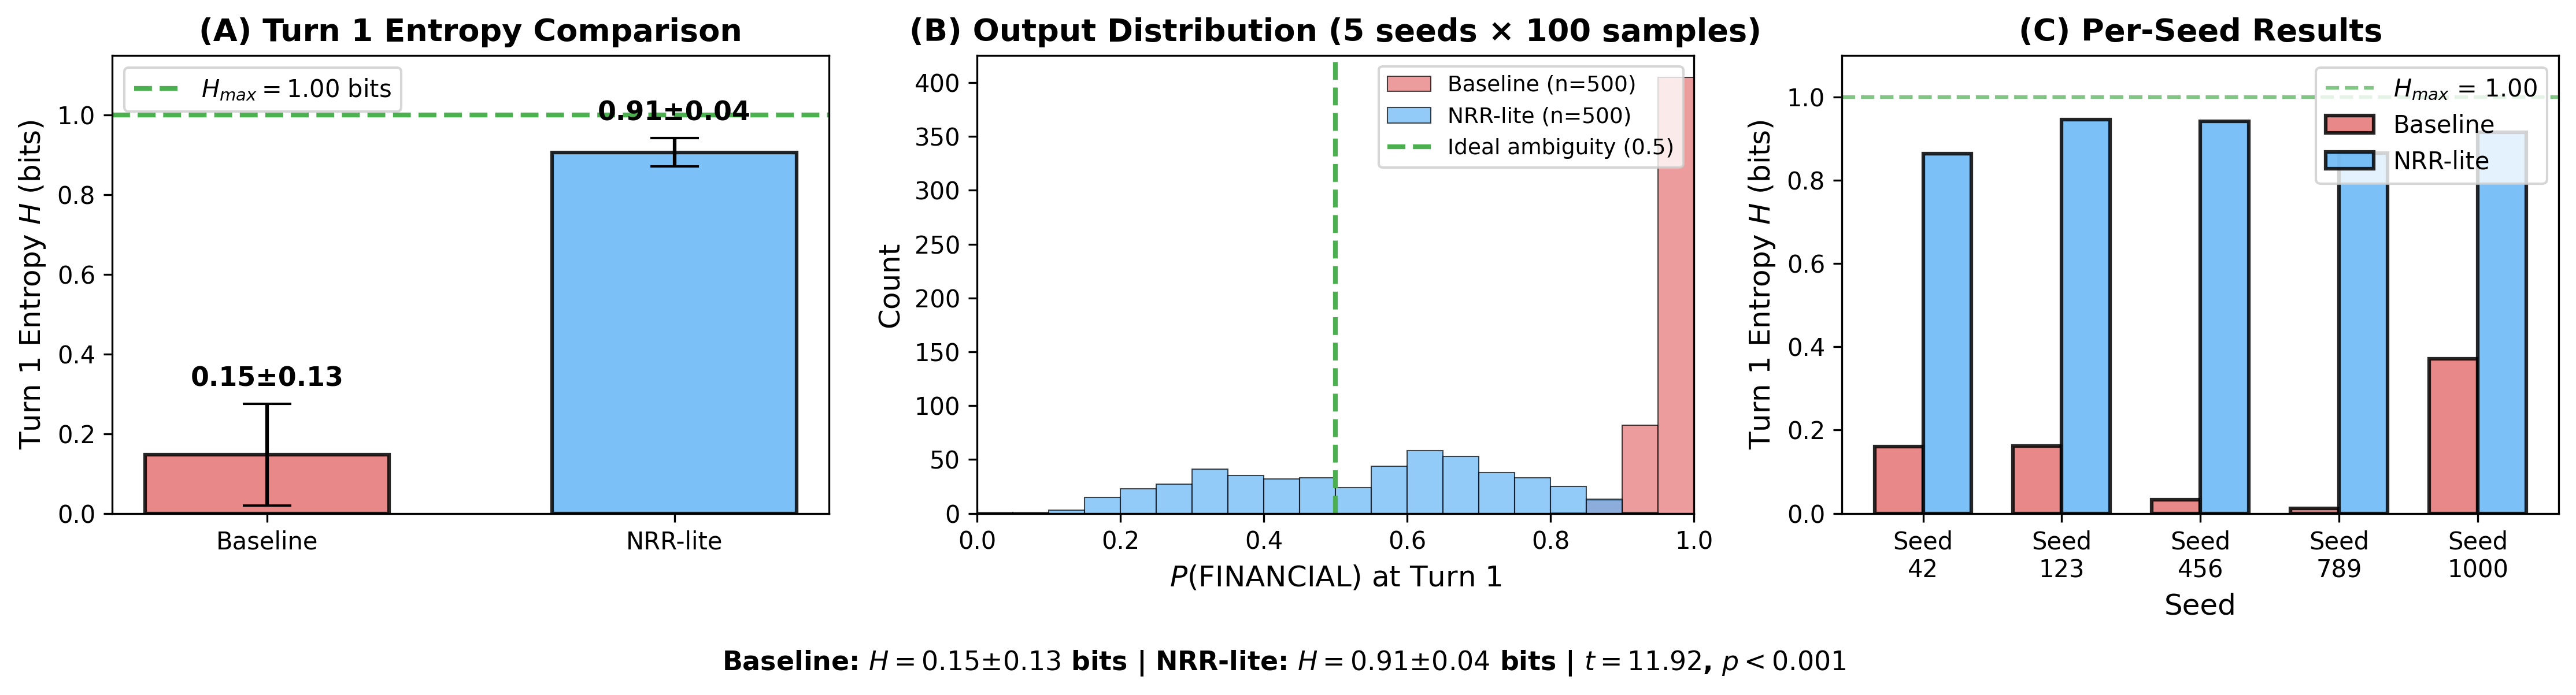
\includegraphics[width=\textwidth]{figure_nrr_experiment.png}
\caption{Turn 1 Entropy Verification Results (aggregated across 5 seeds).
\textbf{Left:} Entropy at Turn 1 (no context). NRR-lite maintains high entropy ($H \approx 0.91$ bits), near the theoretical maximum, while Baseline collapses ($H \approx 0.15$ bits).
\textbf{Center:} Distribution of $P(\text{FINANCIAL})$ at Turn 1 across all test samples (500 total: 5 seeds × 100 samples each). NRR-lite centers around 0.5 (ambiguous); Baseline clusters near 1.0 (committed to financial interpretation).
\textbf{Right:} Per-seed Turn 1 Entropy breakdown across all 5 random seeds, demonstrating consistent preservation by NRR-lite (blue, $H \approx 0.9$ bits across seeds) and variable collapse by Baseline (red, ranging from 0.01 to 0.37 bits depending on initialization).}
\label{fig:nrr_experiment}
\end{figure}

\textbf{Key Findings:}
\begin{enumerate}
    \item \textbf{Baseline Collapse ($H = 0.15$ bits):} The baseline commits to one interpretation at Turn 1, even without disambiguating context. This premature collapse is the architectural bias NRR addresses.
    \item \textbf{NRR-lite Preservation ($H = 0.91$ bits):} NRR-lite maintains near-maximum entropy at Turn 1, confirming that multiple interpretations coexist until context arrives.
    \item \textbf{Gate Behavior:} NRR-lite's context gate achieves $H = 1.0$ bit (perfect balance) when no context is provided, shifting appropriately when Turn 2 arrives.
    \item \textbf{Resolution Capability:} Both models achieve 100\% accuracy with context, demonstrating that ambiguity preservation does not impair eventual resolution.
    \item \textbf{Robustness:} Results replicate across 5 random seeds (paired $t$-test: $t(4) = 11.9$, $p < 0.001$).
    \item \textbf{Baseline Instability:} Baseline's high standard deviation ($\text{SD} = 0.13$, 87\% of mean) reflects architectural instability across random initializations, with entropy ranging from 0.01 to 0.37 bits depending on seed. This contrasts sharply with NRR-lite's consistent performance ($\text{SD} = 0.04$, 4\% of mean), demonstrating robust ambiguity preservation independent of initialization.
\end{enumerate}

This verification provides evidence that NRR-lite implements the $A \neq A$ principle: the same symbol (``bank'') maintains distinct potential identities until context determines which applies.

\section{Future Evaluation Framework}

Comprehensive evaluation requires scaling beyond this minimal verification.
We propose benchmarks for:
\begin{itemize}
    \item \textbf{Ambiguity Retention:} Measuring entropy of interpretations under polysemy.
    \item \textbf{Context-Shift Adaptation:} Measuring cost of adaptation vs. backtracking.
    \item \textbf{Creative Generation:} Human evaluation of semantic richness.
    \item \textbf{Paradox Stability:} Testing system stability under self-reference.
\end{itemize}

\paragraph{Reproducibility note.}
We release the implementation, fixed experiment settings, and primary execution logs in the companion repository.
Core controls are fixed at run time, including model configuration, random seeds, and trial count (temperature is not used in this implementation).
The main paper artifact is generated by the multi-seed command and written as a machine-readable results file.
Exact environment details and command-to-artifact mapping are documented in \texttt{nrr-core/reproducibility.md}.

\section{Conclusion}

This paper introduced \textbf{Non-Resolution Reasoning (NRR)}, a framework challenging classical identity assumptions in AI.
In our controlled setting, we showed that preserving ambiguity can function as a capability rather than a cost.
Our Turn 1 Entropy verification showed that NRR-lite maintains high interpretive entropy ($H = 0.91$ bits) when context is absent, while standard architectures collapse prematurely ($H = 0.15$ bits)---yet both achieve perfect accuracy when context arrives.
NRR challenges the assumption that meaning must collapse to be useful.
The central contribution is operational rather than universal: we make ambiguity-preserving reasoning reproducible and testable under explicit conditions, with boundary/failure regions reported as first-class results.
In this setup, observed gains arise from reducing unnecessary early commitment and preserving reversible update paths, rather than adding architectural complexity.
In this framing, collapse is not rejected; premature collapse is the target failure mode, and commitment is applied when conditions support reliable fixation.
\textbf{The question is not whether AI should resolve ambiguity, but when, how, and under whose control.}

\begin{thebibliography}{99}

\bibitem{devlin2019bert}
Devlin, J., Chang, M. W., Lee, K., \& Toutanova, K. (2019).
BERT: Pre-training of deep bidirectional transformers for language understanding.
\textit{NAACL-HLT}.

\bibitem{peters2018deep}
Peters, M. E., Neumann, M., Iyyer, M., Gardner, M., Clark, C., Lee, K., \& Zettlemoyer, L. (2018).
Deep contextualized word representations.
\textit{NAACL}.

\bibitem{radford2018improving}
Radford, A., Narasimhan, K., Salimans, T., \& Sutskever, I. (2018).
Improving language understanding by generative pre-training.
\textit{Technical report, OpenAI}.

\bibitem{reisinger2010multi}
Reisinger, J., \& Mooney, R. J. (2010).
Multi-prototype vector-space models of word meaning.
\textit{NAACL-HLT}.

\bibitem{levine2020sensebert}
Levine, Y., Lenz, B., Dagan, O., Ram, O., Padnos, D., Sharir, O., Shalev-Shwartz, S., Shashua, A., \& Shoham, Y. (2020).
SenseBERT: Driving some sense into BERT.
\textit{ACL}.

\bibitem{loureiro2022lmms}
Loureiro, D., Jorge, A. M., \& Camacho-Collados, J. (2022).
LMMS Reloaded: Transformer-based sense embeddings for disambiguation and beyond.
\textit{Artificial Intelligence}, 305, 103661.

\bibitem{shazeer2017outrageously}
Shazeer, N., Mirhoseini, A., Maziarz, K., Davis, A., Le, Q., Hinton, G., \& Dean, J. (2017).
Outrageously large neural networks: The sparsely-gated mixture-of-experts layer.
\textit{ICLR}.

\bibitem{child2019generating}
Child, R., Gray, S., Radford, A., \& Sutskever, I. (2019).
Generating long sequences with sparse transformers.
\textit{arXiv preprint arXiv:1904.10509}.

\bibitem{holtzman2020curious}
Holtzman, A., Buys, J., Du, L., Forbes, M., \& Choi, Y. (2020).
The curious case of neural text degeneration.
\textit{ICLR}.

\bibitem{li2023contrastive}
Li, X. L., Holtzman, A., Fried, D., Liang, P., Eisner, J., Hashimoto, T., Zettlemoyer, L., \& Lewis, M. (2023).
Contrastive decoding: Open-ended text generation as optimization.
\textit{ACL}.

\bibitem{goodman2008church}
Goodman, N. D., Mansinghka, V. K., Roy, D. M., Bonawitz, K., \& Tenenbaum, J. B. (2008).
Church: A language for generative models.
\textit{UAI}.

\bibitem{garcez2020neural}
Garcez, A. D., \& Lamb, L. C. (2020).
Neurosymbolic AI: The 3rd wave.
\textit{arXiv preprint arXiv:2012.05876}.

\bibitem{vaswani2017attention}
Vaswani, A., Shazeer, N., Parmar, N., Uszkoreit, J., Jones, L., Gomez, A. N., Kaiser, Ł., \& Polosukhin, I. (2017).
Attention is all you need.
\textit{NeurIPS}.

\bibitem{katharopoulos2020transformers}
Katharopoulos, A., Vyas, A., Pappas, N., \& Fleuret, F. (2020).
Transformers are RNNs: Fast autoregressive transformers with linear attention.
\textit{ICML}.

\bibitem{choromanski2021rethinking}
Choromanski, K., Likhosherstov, V., Dohan, D., Song, X., Gane, A., Sarlos, T., ... \& Weller, A. (2021).
Rethinking attention with performers.
\textit{ICLR}.

\bibitem{dao2022flashattention}
Dao, T., Fu, D. Y., Ermon, S., Rudra, A., \& Ré, C. (2022).
FlashAttention: Fast and memory-efficient exact attention with IO-awareness.
\textit{NeurIPS}.

\bibitem{bachlechner2020rezero}
Bachlechner, T., Majumder, B. P., Mao, H., Cottrell, G., \& McAuley, J. (2020).
ReZero is all you need: Fast convergence at large depth.
\textit{arXiv preprint arXiv:2003.04887}.

\bibitem{ba2016layer}
Ba, J. L., Kiros, J. R., \& Hinton, G. E. (2016).
Layer normalization.
\textit{arXiv preprint arXiv:1607.06450}.
\end{thebibliography}

\section*{Acknowledgments}
The author gratefully acknowledges the support of large language models---including Claude (Anthropic), ChatGPT and Codex (OpenAI), and Gemini (Google)---for their assistance in linguistic refinement, LaTeX formatting, and general proofreading support during the preparation of this manuscript.
All concepts, arguments, and conclusions remain solely the responsibility of the author.

\end{document}
